% Primarily this section should be about scientific methods and theories you need to evaluate/compare/invent to solve your problems from 1.3.
% In some cases it may be ok to describe different technologies, but the purpose is to describe something and then draw a conclusion from that.
% Example, if you decide to discuss different databases, it may be for the purpose of selecting the best type for your implementation later on (based on for example data representation, scalability, speed, etc.).
% Optimally the problems in 1.3 are not solved by anyone else yet, in which case this section needs to describe how to solve them (new algorithms, mathematical approaches, etc.).
 
% This section can have a lot of subsections (3.1, 3.2, 3.3, etc).

The values of a computer program needs to be temporary stored somewhere on the computer were they can easily be access while running the program.
The two main ways the computer can do this is to either store values in registers or in the memory.
Registers are very limited in space and are very volatile thus they are good for storing values which are used many times in a short amount of time.
Memory is much slower but has a lot more space.
Memory is thus much more useful for storing values that are not needed right now but will be needed in the future.


It is the compiler that decide when and if a variable will be stored in registers or memory.
The compiler decides this when compiling the computer program, which means the developer has usually very little control over where the values are stored.


Values stored in memory are either stored on the call stack or the heap.
The call stack holds all the arguments and variables for all the called functions that have not finished execution.
While the heap contain all the dynamically allocated values.


\subsubsection{Registers}
Computer registers are small memory spaces that are of fixed size.
These registers can store any type of data as long as it fits within the size limit of the registers.
Some of the registers are reserved for special use, one of the most important ones is the \acrfull{pc} register.
This register always holds the address of the next machine code instruction that will be executed.
Which of the registers that are reserved for special use is different depending on the processor.


\subsubsection{Call Stack}
The call stack is a stack in the memory that has the arguments and variables of all the functions that have been called and are not finished executing.
A stack is a data structure that consist of a number of elements that are stacked on top of each other and the only two operations available for a stack is push and pop.
The push operations adds a new element on top of the stack and the pop operation removes the top element of the stack.
Other key characteristics are that it is only the top element that can be accessed, thus to reach the lower elements, all the above elements needs to be popped.


Stack/call frames are the elements that make up the call stack, each stack frame has the values of the arguments and variables for one function call.
Stack frames also usually contain a return address which is pointer to a machine code instruction, this instruction is the next instruction of the previous function that called the current function.
When a function has finished executing its stack frame will be pop/removed from the stack and the previous function will continue executing. 
An example of a call stack and stack frames can be seen in the figure \ref{fig:callstack}.


\begin{figure}[h]
	\centering
	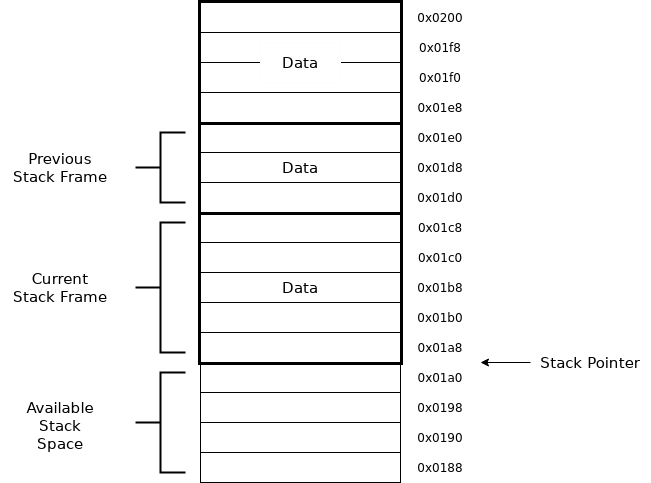
\includegraphics[width=1.0\textwidth]{call-stack.png}
	\caption{An visual example of how a stack and stack frames can look.}
	\label{fig:callstack}
\end{figure}


%\subsubsection{Heap}
%TODO

